\section{Introduction}

Advances in hardware that augment a user's physical actions have reignited dreams of overcoming human limitations, recovering lost abilities and simplifying skill acquisition~\citep{Goto2020-mw, Kunze2017-co}. These technological advances include the miniaturization of the actuating hardware to wearable form factors and the direct sensing and stimulation capabilities of neural interfaces. Especially due to these characteristics, recent perspectives promote a change of the computing era from human-computer \textit{interaction} to \textit{integration}~\cite{Mueller2020-dl}. One key change in perspective is, that \textit{integrated} users share agency with the computing machinery to execute tasks. This is a critical distinction as \textit{integration} technologies are designed to directly influence people’s bodies, their actions, and the resulting action outcomes.

Besides body and outcome augmentation, action augmentation has been defined as the case where a ``system assists the user’s action to produce the intended outcome.''~\cite{Cornelio2022-aq}. Such action augmentations can be realized purely on a software integration level, for example by an AI pair programmer. When it is designed to happen on a hardware level, further challenges emerge, specifically due to shared agency, which in this case means handing over control of one's body. Unfortunately, such augmented users often report dissociative experiences, frequently disrupting their sense of agency (SoA)~\citep{Gilbert2017-ze, Gilbert2019-uc}.


Having a SoA means experiencing control of our own voluntary actions, instead of them feeling as randomly happening to us. It has been shown that users are more likely to feel engaged and satisfied with an interaction, and are more likely to trust a system the more they experience SoA~\citep{Berberian2012-do, Miller2007-rb}. Hence, a key challenge to drive the adoption of human action augmentation is to design for agency experience, so users feel as though they are in the ``driver's seat'' once again.

\subsection{Preserving Agency using Brain Signals of the Intent to (Inter-) act}
In this paper, we present a prototype to overcome the disruption in experiencing agency during action augmentation. We developed a brain-computer interface (BCI) that establishes a fast communication channel between a user's brain signals and a physical end effector. The augmentation system (from hereon referred to simply as \textit{system}) controls the user's muscles at the time of their \textit{intent to interact}, as measured through readiness potentials (RP) manifesting in the user's electroencephalogram (EEG)~\cite{Schurger2021-vp, Schultze-Kraft2016-bx, Schultze-Kraft2021-cu}. 

\begin{figure}[!h]
    \centering
    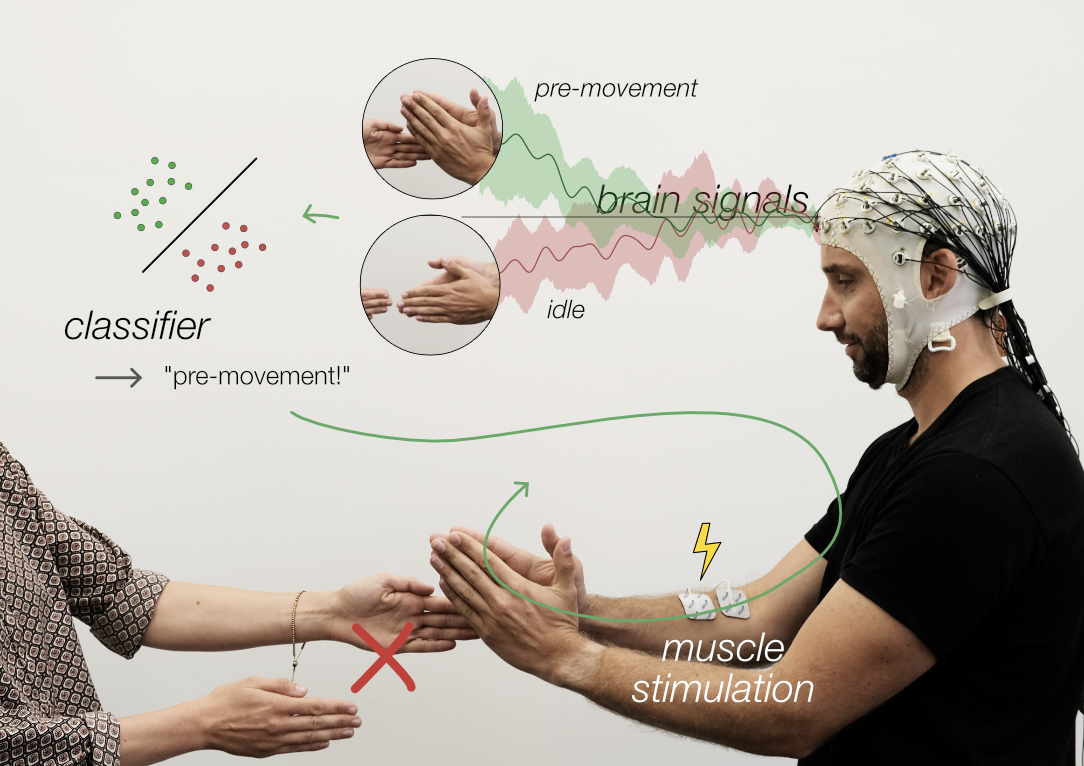
\includegraphics[width=\columnwidth]{figures/teaser_new.png}%{figures/bci_game.png}
    \caption{Our augmentation system: When participants feel the spontaneous urge to move, readiness potentials (RPs) are picked up in the user's brain signals. A brain-computer interface (BCI) predicts the data to be in either of two classes: Idle or pre-movement. In the latter case, electrical muscle stimulation (EMS) is triggered and the user's hand is moved. Image taken with consent from participant.}
\end{figure}

To control the interaction in real-time, an RP-based classifier distinguished between two user states: \textit{idle}, reflecting the absence of an intent to act, and \textit{pre-movement}, indicating the presence of an intent to act. During \textit{idle}, participants were passively looking at a fixation cross. Instead, during \textit{pre-movement}, participants were instructed to voluntarily initiate a tap on a touchscreen whenever they felt the urge to do so. Previous work has indicated that the RP emerges during formation of conscious intention and is specific to voluntary action~\cite{Schultze-Kraft2020-rm, Travers2020-hf, Pares-Pujolras2019-ll}.

Upon predicting a \textit{pre-movement} state, the system augmented the user's action, potentially preceding their voluntary motor command. This augmentation moved the ring finger in accordance with the user's intention to act. We achieved the movement by leveraging electrical muscle stimulation (EMS) applied to the user's forearm flexor muscle. In our user study, a mixed-methods research approach was employed to explore whether aligning the physical impact on the user's body with their intention to move preserved their SoA.



